\subsection{Data Analysis}
Our analysis was limited to data from participants who reported using 9 to 10 fingers to type, as these participants were more likely to adhere to touch typing practices. Touch typing is a standardized method in which typists use muscle memory to locate keys without looking at the keyboard, and it is the most common method of typing among proficient typists. Although users may deviate from perfect touch typing in practice, this approach enables a systematic examination of typing patterns while still reflecting real-world usage.

\subsubsection{Bistroke Analysis}
\noindent The bistroke analysis reveals that frequency is the most significant predictor of typing time. As illustrated in Figure \ref{fig:freq_to_time}, typing speed follows a logarithmic curve with frequency, indicating that muscle memory aids high-frequency bistrokes regardless of placement. Once the impact of frequency is accounted for, the effect of key placement and the positional relationships between keys can be examined. As expected, the analysis shows that finger dexterity plays a role in typing speed, with the pinkies being the slowest and the index and middle fingers being the fastest. Notably, the top row is predicted to be marginally faster than the home row. This could be a bias in the data, as the top is the most used row on QWERTY, QWERTZ, and AZERTY, three of the four layouts analyzed. Further analysis is required to determine whether the slight advantage of the top row arises from an inherent biomechanical ease of movement when the fingers operate closer to their natural midpoint of flexion or if it reflects learned behavior. Analyzing the positional relationships between keys reveals three major categories of bistrokes:

\begin{itemize}
  \item \textbf{ALT (Alternating Bistroke):} a bigram typed by alternating hands. This is the fastest bistroke category as little coordination is needed to articulate the movement.
\item \textbf{SHB (Single-hand Bistroke):} a bigram typed with the same hand. This category is typically slower due to the need for sequential finger movements on the same hand and, therefore, greater coordination.
\item \textbf{SFB (Single-finger Bistroke):} A bigram typed using the same finger in succession. This is the slowest category, requiring both high coordination and inherent downtime. SFBs are especially slow at high words per minute.
\end{itemize}

\noindent The key finding of this analysis is that the impact of a feature on speed prediction depends on the WPM range of the data used. This is clearly demonstrated by the effect of the WPM range on SFBs, which become significantly worse at high WPMs. This observation underscores the need to tailor keyboard optimization to specific typing speed goals, which in turn complicates both decision-making in the layout creation process and the implementation of the simulated annealing algorithm.

\begin{figure}[h]
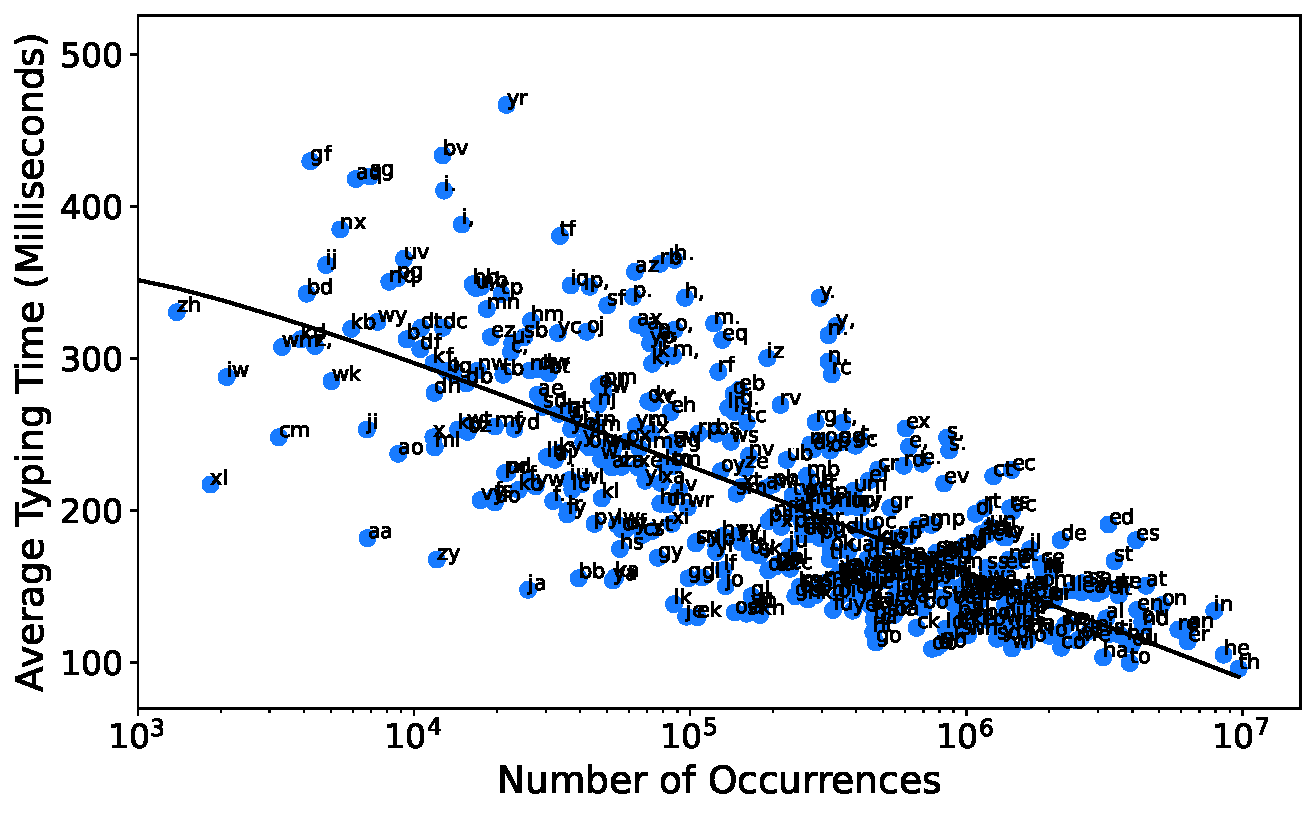
\includegraphics[width=\columnwidth]{figures/freqplot.pdf}
\caption{Relationship Between English Bigram Frequency and Average Typing Time on QWERTY}
\label{fig:freq_to_time}
\end{figure}

\begin{figure}[h]
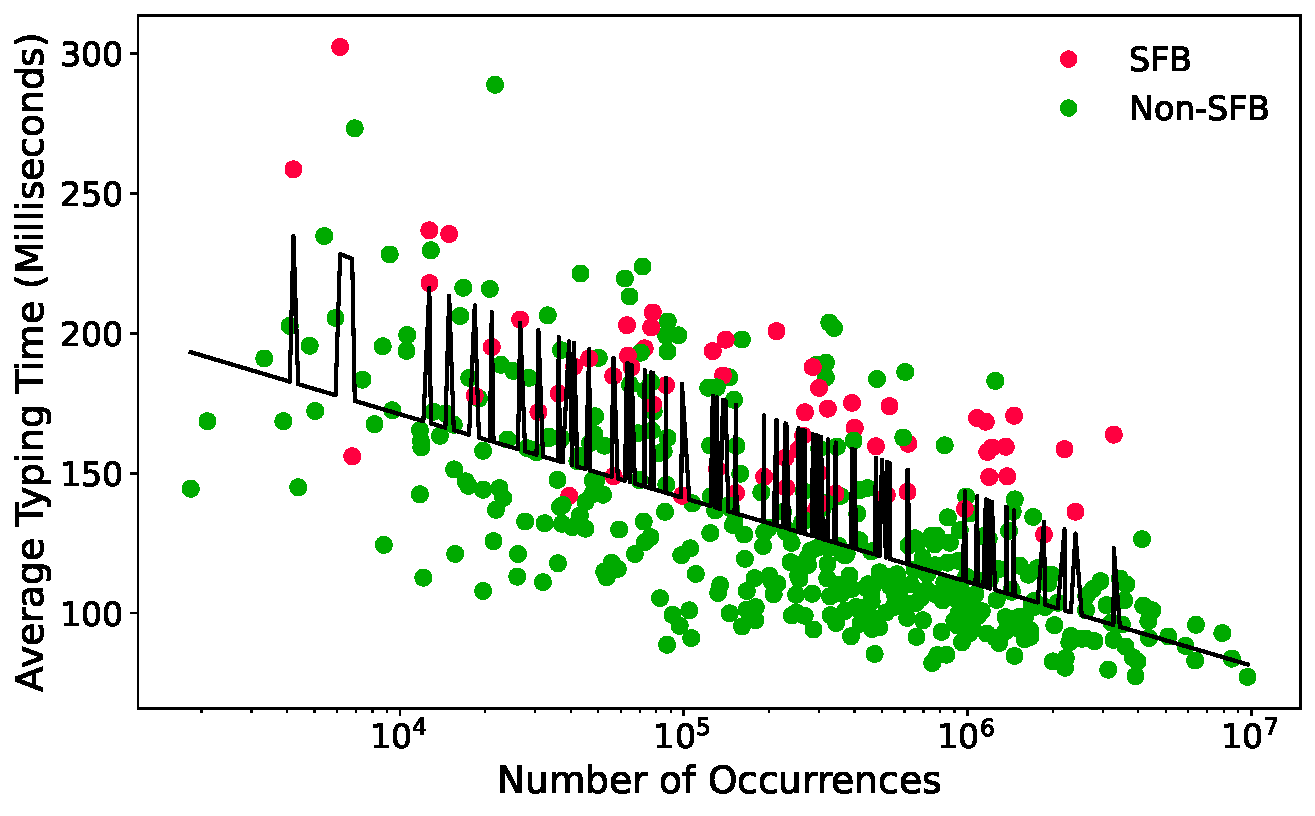
\includegraphics[width=\columnwidth]{figures/sfbplot.pdf}
\caption{The Effect of SFBs and Frequency on Typing Time ($>80$WPM)}
\label{fig:bigram_typing_time}
\end{figure}

\subsubsection{Tristroke Analysis}
\noindent Several features unique to tristrokes were identified; however, they were excluded from the analysis due to their low statistical significance and the increased risk of overfitting the model. The only exception to this exclusion is the single-finger skipstroke category. Single-finger skipstrokes, like single-finger bistrokes, involve two strokes made by the same finger, but with an intervening stroke between them. An example of this on the QWERTY keyboard is the word "fit," as both the 'f' and 't' are typed with the left index finger, leading to a coordinative delay. Single-finger skipstrokes are important to consider because, for fast typists, they function similarly to single-finger bistrokes with an added delay. Since single-finger bistrokes notably impact typing speed -- especially at higher typing speeds -- accounting for single-finger skipstrokes is imperative when targeting faster typing speeds.



 %  and may be important for different models
% Tristroke analysis merits future exploration.
% Time prediction for tristrokes is performed by taking the sum of the tristroke's constituent bistrokes and adding a small as they make up most of the time fluctuations associated with a given tristroke.